\section*{Introduction}
Dans ce chapitre, nous observerons les différentes avancées qui ont déjà eues lieues dans le domaine de la transcription automatique de la musique et de la batterie afin de situé notre démarche.\\
Nous aborderons le passage crucial du monophonique au polyphonique dans la transcription. Nous ferons un point sur les deux grandes parties de l’AMT de bout en bout : de l’audio vers le MIDI puis des données MIDI vers l’écriture d’une partition. Ensuite, nous ferons une critique des approches linéaires et des approches hiérarchiques. Enfin, nous ferons un bilan afin de situer l’ADT dans l’état de l’art de l’AMT.
  
\section{Monophonique et Polyphonique}
\begin{itemize}
	\item ref systèmes polyvalents richesse des sons.\\
\end{itemize}
Les premiers travaux ont été faits sur l’identification des instruments monophoniques\footnote{Une seule note à la fois, ou plusieurs notes de même durée (monophonie par accord).}\cite{future_directions}. Actuellement, le problème de l'estimation automatique de la hauteur des signaux monophoniques peut être considéré comme résolu, mais dans la plupart des contextes musicaux, les instruments sont polyphoniques.\\
L'estimation des hauteurs multiples (détection multi-pitchs ou F0 multiples) est le problème central de la création d'un système de transcription de musique polyphonique. Il s’agit de la détection de notes qui peuvent apparaître simultanément et être produites par plusieurs instruments différents. Ce défi est donc majeur pour la batterie puisque c’est un instrument qui est lui-même constitué de plusieurs instruments.\\
Le fort degrés de chevauchement entre les durées ainsi qu’entre les fréquences complique l’identification des instruments polyphoniques. Cette tâche est étroitement liées à la séparation des sources et concerne aussi la séparation des voix. Les performances des systèmes actuels ne sont pas encore suffisantes pour permettre la création d'un système automatisé capable de transcrire de la musique polyphonique sans restrictions sur le degré de polyphonie ou le type d'instrument. Cette question reste donc encore ouverte. 
\section{Audio vers MIDI}
Utilité de l’audio vers MIDI dans la vraie vie $\Rightarrow$ p. 4 et 5 de \cite{Review_ADT}.\\\\
La plupart des travaux se sont concentrés sur le traitement du signal vers la génération du midi \cite{AMT_for_2_Instru}. Cette partie plusieurs sous-tâches dont la détection multi-pitchs, la détection des onset et des offset, l'estimation du tempo, la quantification du rythme, la classification des genres musicaux,…\\\\
En ADT\cite{Review_ADT}, plusieurs stratégies de répartition Pre/Post-processing sont possibles pour la détection multi-pitchs. Une des démarches intuitives serait de la préparer dès le préprocessing, dans le pré-traitement, pendant la séparation des sources en supprimant les features non-pertinentes pour une meilleure détection des instruments de la batterie. Par exemple, en supprimant la structure harmonique pour atténuer l’influence des instruments à hauteurs sur la détection grosse-caisse et caisse-claire. Mais certaines études montrent que des expériences similaires ont donné des résultats non-concluants et que la suppression des instruments à hauteurs peut avoir des effets néfastes sur les performances de l’ADT. Cependant, les systèmes d’ADT basés sur des RNN ou des NMF font la séparation des sources pendant l’optimisation ce qui réduit la nécessité de la faire pendant le préprocessing.\\
Pour la reconnaissance des instruments, une approche possible\cite{Eronen} est de mettre un modèle probabiliste dans l’étape de la classification des évènements afin de classer les différents sons de la batterie. Dans cette méthode, on se place de sample audio isolés en modélisant la progression temporelle des features avec un HMM. Les features sont transformés en représentations statistiques indépendantes.
L’approche AdaMa\cite{adama_1} est une autre approche de la même catégorie, elle commence par une estimation initiale des sons de la batterie qui sont itérativement raffinés pour matcher l’enregistrement visé.\\
- Extraction of rhythmic information (tempo, beat, and musical timing)\\
\section{MIDI vers partition}
Lorsque les travaux principaux parlent de transcription de bout en bout, l’appellation « score » (\textit{partition}) désigne souvent un ouput au format Music XML, ou simplement MIDI. Par exemple, dans \cite{SHIBATA2021262}, la chaîne de traitement va jusqu’à la génération d’une séquence MIDI quantifiée qui est importée dans MuseScore pour en extraire manuellement un fichier MusicXML contenant plusieurs voix.\\
Seuls quelques travaux récents s’intéressent de près à la création d’outils permettant la génération de partition. Le problème de la conversion d'une séquence d'événements musicaux symboliques en une partition musicale structurée est traité notamment dans \cite{foscarin:hal-01988990}. Ce travail, qui vise à résoudre en une fois la quantification du rythme et la production de partition, s’appuie tout au long du processus sur  des grammaires génératives qui fournissent un modèle hiérarchique à priori des partitions. Les expériences ont des résultats prometteurs, mais il faut relevé qu’elle ont été menées avec un ensemble de données composé d'extraits monophoniques, il reste donc a traiter le passage au polyphonique en couplant le problème de la séparation des voix avec la quantification du rythme.\\
L'approche de \cite{foscarin:hal-01988990} est fondée sur la conviction que la complexité de la structure musicale dépasse les modèles linéaires.
\section{Approche linéaire et approche hiérarchique}
%\subsection*{Approche linéaire}
Plusieurs travaux ont d’abord privilégié l’approche stochastique. Par exemple, Shibata et al.\cite{SHIBATA2021262} ont utilisé le modèle de Markov caché (HMM)\footnote{\url{https://fr.wikipedia.org/wiki/Modèle_de_Markov_caché}}\footnote{\url{https://en.wikipedia.org/wiki/Hidden_Markov_model}} pour la reconnaissance de la métrique. Ils utilisent d’abord deux réseaux de neurones profonds, l’un pour la reconnaissance des pitchs et l’autre pour la reconnaissance de la vélocité. Pour la dernière couche, la probabilité est obtenue par une fonction sigmoïde. Ils construisent ensuite plusieurs HMM métriques étendus pour la musique polyphonique correspondant à des métriques possibles et ils calculent la probalitité maximale pour chaque modèle afin d’obtenir la métrique la plus probable.
\begin{figure}[h]
	\centering
	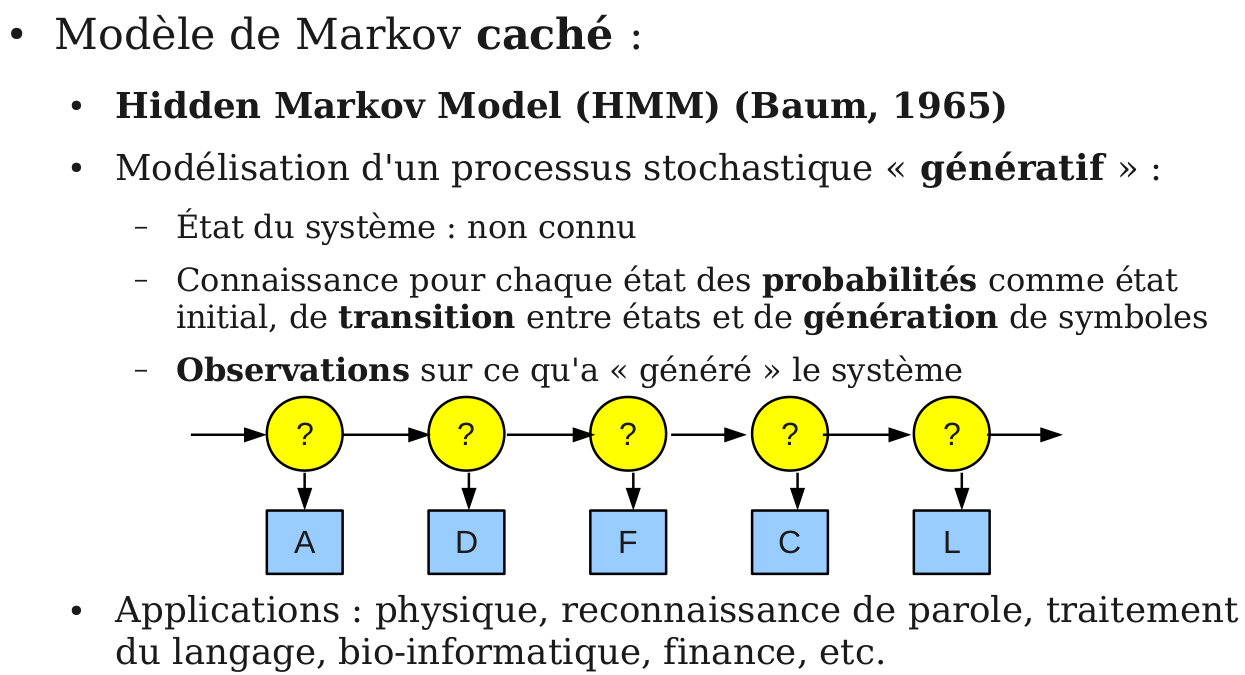
\includegraphics[height=50mm, width=90mm]{z_images/2_etat_de_l_art/hmm.png}
	\caption{HMM}
	\textit{Source : Cours de Damien Nouvel\footnote{\url{https://damien.nouvels.net/fr/enseignement}}}
\end{figure}

L’évaluation finale des résultats de \cite{SHIBATA2021262}, montre qu’il faut rediriger l’attention vers les valeurs des notes, la séparation des voix et d'autres éléments délicats de la partition musicale qui sont significatifs pour l'exécution de la musique. Hors de nombreux travaux suggèrent d’utiliser une approche hiérarchique puisque le langage musical est lui-même structuré hiérarchiquement. En effet, ces structures (notamment les arbres syntaxiques) sont idéals pour représenter le langage musical.
\subsection*{Approche hiérarchique}
La nécessité d’une approche hiérarchique pour la production automatique de partition est évoquée dans \cite{foscarin:hal-01988990} même si la quantification du rythme se fait le plus souvent par la manipulation de données linéaires allant notamment des real time units (secondes) vers les musical time units (temps, métrique,…).\\
Dans \cite{foscarin:hal-01988990}, les modèles de grammaire exposés sont différents de modèles markoviens linéaires de précédent travaux.\\\\
Image qui provient de \cite{harasimjazz} :\\
\begin{figure}[h]
	\centering
	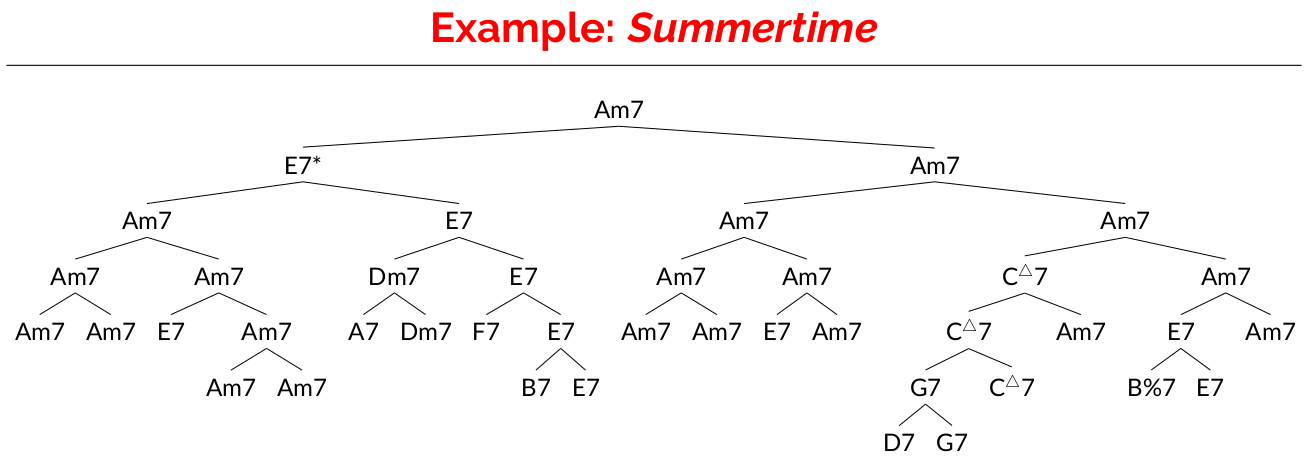
\includegraphics[height=40mm, width=120mm]{z_images/2_etat_de_l_art/summertime_tree.png}
\end{figure}\\

\cite{rohrmeier2020towards} cherchent à caractériser la structure interne récursive des rythmes musicaux en utilisant une grammaire formelle.
Cela va au-delà du GTTM (?), qui ne propose pas de modèle du rythme, et soutient en outre que l'inférence de la structure rythmique hiérarchique profonde est centrale à la cognition musicale. En raison de la représentation conjointe de la structure rythmique et métrique dans le modèle, un analyseur syntaxique de la grammaire abstraite du rythme musical proposée instancie l'interprétation rythmique et l'inférence métrique en même temps.\\\\
et nous montrerons que l’approche hiérarchique est plus adapté au traitement de la musique dont l’écriture est une structure hiérarchique en soi.
\section{Bilan sur l’ADT}
\begin{itemize}
	\item Personne fait du MIDI vers partition ;
	\item Pas de formalisation de la notation de la batterie ;
	\item bla bla…
\end{itemize}
Un grand nombre travaux ont déjà été menés dans le domaine de l’ADT. La plupart ont été énumérés par Wu et al. \cite{Review_ADT} qui, pour mieux comprendre la pratique des systèmes d’ADT, se concentrent sur les méthodes basées sur la factorisation matricielle non négative et celles utilisant des réseaux neuronaux récurrents.\\
\section*{Conclusion}
La plupart des travaux déjà entrepris se concentrent sur des méthodes de calcul pour la détection d'événements sonores de batterie à partir de signaux acoustiques ou sur la séparation entre les évènement sonore de batterie avec ceux des autres instruments dans un orchestre ou un groupe de musique \cite{2802}, ainsi que sur l'extraction de caractéristiques de bas niveau telles que la classe d'instrument et le moment de l'apparition du son. Très peu d'entre eux ont abordé la tâche de générer des partitions de batterie.
Nous avons décidé de compléter le travail qui concerne la batterie en commençant par l’endroit le moins pratiqué, à savoir la transcription du MIDI vers la partition.